
\begin{abstract}
Evaluating probabilistic forecasts is complex and essential across various domains, yet no comprehensive software framework exists to simplify this task. Despite extensive literature on evaluation methodologies, current practices are fragmented and often lack reproducibility. To address this gap, we introduce a reproducible experimental workflow for evaluating probabilistic forecasting algorithms using the sktime package. Our framework features a unified software API for forecasting algorithms, a simple specification language for complex algorithms, including meta-algorithms like bootstrapping, probabilistic performance metrics, and standardized evaluation workflows. We demonstrate the framework's efficacy through a study evaluating prediction intervals added to point forecasts. Our results highlight the improved prediction accuracy and reliability of combined approaches. We provide reusable code and invite contributions from the research community to extend our experiments and tackle computational challenges for broader studies.

\end{abstract}

\section{Introduction}\label{introduction}
Making probabilistic forecasts is challenging, and evaluating probabilistic forecasts, or the algorithms that produce them, is even more difficult. 

A significant body of literature focuses on developing robust meta-methodologies for evaluation. This includes evaluation metrics such as the Continuous Ranked Probability Score (CRPS) \cite{gneiting2014probabilistic} and their properties, like properness, as well as benchmarking setups and competitions like the Makridakis competitions \cite{makridakis2020_m4, makridakis2022_m5}. This meta-field builds upon a broader primary field that develops methodologies for algorithms producing probabilistic forecasts, encompassing classical methods, uncertainty estimation techniques like bootstrap or conformal intervals, and modern deep learning and foundation models \cite{chen2020probabilistic, nowotarski2018probabilistic, lagllama, decoder_foundation_forecasting}.

Despite the critical importance of evaluating probabilistic forecasts in various domains, including finance, energy, healthcare, and climate science, no comprehensive software framework or interface design has emerged to cover all these needs with a simple workflow or specification language. For instance, the reproducing code for the Makridakis competitions—while extensive in scope—relies on forecasts generated from disparate software interfaces. Similar issues are found in other benchmarking studies, where code availability is often limited or nonexistent. This lack of unified interfaces makes it challenging for practitioners in both industry and academia to contribute to or verify the growing body of evidence.

To address these limitations, we present a simple, reproducible experimental workflow for evaluating probabilistic forecasting algorithms using \texttt{sktime} \cite{franz_kiraly_2024_11095261_sktime}. As of 2024, the \texttt{sktime} package provides the most comprehensive collection of time series-related algorithms in unified interfaces and stands out as the only major, non-commercially governed framework for time series forecasting.

The key components of this reproducible benchmarking framework are:

\begin{itemize}
  \item A unified software API for forecasting algorithms, mirroring a unified mathematical interface.
  \item Composite forecasters (meta-algorithms), such as adding prediction intervals via time series bootstrapping, which themselves follow the same forecasting interface from both software and mathematical perspectives.
  \item A first-order language that allows for the unambiguous specification of even complex forecasting algorithms.
  \item A unified software API for probabilistic performance metrics, covering metrics for distribution as well as interval or quantile forecasts.
  \item A standardized workflow for obtaining benchmark result tables for combinations of algorithms, metrics, and experimental setups.
\end{itemize}

To demonstrate the efficacy and ease of use of \texttt{sktime} in benchmarking probabilistic forecasters, we conducted a small study exploring the performance of various meta-algorithms (wrappers) that add prediction intervals to point forecasters. We investigated a range of forecasters, including Naive Forecasting and AutoTheta models \cite{autotheta}, along with probabilistic wrappers such as Conformal Intervals and Bootstrapping Methods. The study's goal was to evaluate the effectiveness of these combined approaches in improving prediction accuracy and reliability.

We conducted experiments on several common datasets, including Australian electricity demand \cite{Godahewa2021Australian}, sunspot activity \cite{Godahewa2021Sunspot}, and US births \cite{Godahewa2021USBirth}. These datasets represent different time frequencies and characteristics.

Our paper is accompanied by easily reusable code, and we invite the open research and open-source communities to contribute to extending our experiments or using our code to set up their own. As is often the case in modern data science, computational power is a limiting factor, so we hope to leverage the SciPy conference to plan a more comprehensive set of studies.

The remainder of this paper is organized as follows: In Section \ref{methods}, we describe the forecasting methods and probabilistic wrappers used in our experiments. Section \ref{datasets} provides an overview of the datasets used for evaluation. In Section \ref{results}, we present the experimental results and discuss the performance of the combined approaches. Finally, in Section \ref{conclusion}, we conclude the paper and outline directions for future research.

\section{sktime and tsbootstrap for Reproducible Experiments}\label{sktime}

In this section, we summarize the key design principles used for reproducible benchmarking in \texttt{sktime}.

\subsection{Unified Interface}
In \texttt{sktime} and \texttt{tsbootstrap}, algorithms and mathematical objects are treated as first-class citizens. All objects of the same type, such as forecasters, follow the same interface. This consistency ensures that every forecaster is exchangeable with any other.

Forecasters are objects with \texttt{fit} and \texttt{predict} methods, allowing both the target time series (endogenous data) and the time series that influence the target time series (exogenous data) to be passed. For example, the following code specifies a forecaster, fits it, and makes predictions.

\begin{verbatim}
# importing the necessary modules
from sktime.datasets import load_airline
from sktime.forecasting.naive import NaiveForecaster

# load exemplary data
y = load_airline()

# specifying the forecasting algorithm
forecaster = NaiveForecaster(strategy="last", sp=12)

# fitting the forecaster -- forecast y into the future, 3 steps ahead
forecaster.fit(y, fh=[1, 2, 3])

# querying predictions
y_pred = forecaster.predict()
\end{verbatim}

A crucial design element in the above is that the first line can specify any forecaster - for instance, \texttt{ARIMA} or \texttt{ExponentialSmoothing},
and the rest of the code will work without modification.

This design pattern is consistent across all forecasters in \texttt{sktime}, and called the "strategy pattern" in software engineering.

Currently, \texttt{sktime} supports the construction of 82 individual forecasters, either implemented within the package or interfaced from other packages in the ecosystem. Each forecaster is parametric, with configurations ranging from 1 to 47 parameters across different forecasters. A list of forecasters can be obtained or filtered via the \texttt{all\_estimators} utility.
To better filter the forecasters (as well as the other estimators such as classifiers and regressors) based on their properties and capabilities and to control their behaviour, \texttt{sktime} implements a tag system. Each estimator, such as a forecaster, has a dict \texttt{\_tags}, with a string as a key describing the name and a value of an arbitrary type describing the property.

This type system enables an easy identification of all probabilistic forecasters, since they are tagged with the \texttt{"capability:pred\_int"} tag. Currently, 45 of the 82 forecasters support probabilistic prediction modes, such as prediction intervals, quantile predictions, or full distributional predictions:

\begin{verbatim}
# importing the necessary modules
from sktime.datasets import load_airline
from sktime.forecasting.naive import NaiveForecaster

# load exemplary data
y = load_airline()

# specifying the forecasting algorithm
forecaster = NaiveForecaster(strategy="last", sp=12)

# fitting the forecaster -- forecast y into the future, 3 steps ahead
forecaster.fit(y, fh=[1, 2, 3])

# making interval predictions
y_pred_int = forecaster.predict_interval()
# making distribution predictions
y_pred_proba = forecaster.predict_proba()
\end{verbatim}

More details can be found in the official tutorials (an overview of notebooks and tutorials is provided on our \href{https://www.sktime.net/en/latest/users.html}{homepage}).
Creating algorithms with compatible APIs is straightforward.

\texttt{sktime} and \texttt{tsbootstrap} provide fill-in \href{https://github.com/sktime/sktime/tree/main/extension_templates}{extension templates} for creating algorithms in a compatible interface, which can be shared in a third-party code base and indexed by \texttt{sktime}, or contributed directly to \texttt{sktime}.

\subsection{Reproducible Specification Language}
All objects in \texttt{sktime} are uniquely specified by their construction string, which serves as a reproducible blueprint. Algorithms are intended to be stable and uniquely referenced across versions; full replicability can be achieved by freezing Python environment versions and setting random seeds.

For example, the specification string 
\texttt{NaiveForecaster(strategy="last", sp=12)}
uniquely specifies a native implementation of the seasonal last-value-carried-forecaster, with seasonality parameter 12.

Typical \texttt{sktime} code specifies the forecaster as Python code, but it can also be used as a string to store or share specifications. The \texttt{registry.craft} utility converts a Python string into an \texttt{sktime} object, ensuring easy reproducibility:

\begin{verbatim}
from sktime.registry import craft
forecaster = craft('NaiveForecaster(strategy="last", sp=12)')
\end{verbatim}
which can be used to copy a full specification from a research paper and immediately construct the respective algorithm in a Python environment, even if full code has not been shared by the author.

This approach makes it extremely easy to share specifications reproducibly, simplifying the often convoluted process of describing algorithms in research papers.

\subsection{Meta-Algorithms and Composability}
\texttt{sktime} provides not only simple algorithms as objects in unified interfaces but also meta-algorithms, such as data processing pipelines or algorithms that add interval forecast capability to existing forecasting algorithms. Importantly, these composites also follow unified interfaces.

This leads to a compositional specification language with rich combinatorial flexibility. For example, the following code adds conformal prediction interval estimates to the \texttt{NaiveForecaster}:

\begin{verbatim}
# importing the necessary modules
from sktime.datasets import load_airline
from sktime.forecasting.naive import NaiveForecaster
from sktime.forecasting.conformal import ConformalIntervals

# load exemplary data
y = load_airline()

# specifying the forecasting algorithm
forecaster = ConformalIntervals(NaiveForecaster(strategy="last", sp=12))

# fitting the forecaster -- forecast y into the future, 3 steps ahead
forecaster.fit(y, fh=[1, 2, 3])

# making interval predictions
y_pred_int = forecaster.predict_interval()
\end{verbatim}

The conformal prediction interval fits multiple instances of the wrapped forecaster on on parts of the time series using window sliding. In particular, each forecaster's instance $i$
is fit on the time series $y_{1:t_i}$, where $t_i \neq t_j$. Afterwards, the residuals are computed on the remaining time series $y_{t_{i+1}:n}$, where $n$ is the length of the time series.
Out of these residuals, the prediction intervals are computed.
The resulting algorithm possesses \texttt{fit}, \texttt{predict}, and - added by the wrapper - \texttt{predict\_interval}, as well as the \texttt{capability:pred\_int} tag.

Data transformation pipelines can be constructed similarly, or with an operator-based specification syntax:

\begin{verbatim}
# importing the necessary modules
from sktime.datasets import load_airline
from sktime.forecasting.naive import NaiveForecaster
from sktime.transformations.series.detrend import Deseasonalizer
from sktime.transformations.series.difference import Differencer

# load exemplary data
y = load_airline()

pipeline = Differencer() * Deseasonalizer(sp=12) * NaiveForecaster(strategy="last")

# fitting the forecaster -- forecast y into the future, 3 steps ahead
pipeline.fit(y, fh=[1, 2, 3])

# making interval predictions
y_pred_int = pipeline.predict()
\end{verbatim}

This creates a forecasting algorithm that first computes differences, then remove the seasonality (deseasonalize) by assuming a periodicity of 12, 
then the \texttt{NaiveForecasster(strategy="last")} uses the last value as prediction for the next values (last-value-carry-forward method), finally it adds the seasonality back
and inverts the first differences.
As before, the resulting forecaster provides unified interface points and is interchangeable with other forecasters in \texttt{sktime}.

\subsection{Probabilistic Metrics}
In \texttt{sktime}, evaluation metrics are first-class citizens. Probabilistic metrics compare the ground truth time series with predictions, representing probabilistic objects such as predictive intervals or distributions. For example:

\begin{verbatim}
# importing the necessary modules
from sktime.datasets import load_airline
from sktime.forecasting.naive import NaiveForecaster
from sktime.performance_metrics.forecasting.probabilistic import CRPS
from sktime.split import temporal_train_test_split

# load exemplary data
y = load_airline()
y_train, y_test = temporal_train_test_split(y, test_size=36)

# specifying the forecasting algorithm
forecaster = NaiveForecaster(strategy="last", sp=12)

# fitting the forecaster -- forecast y into the future, 3 steps ahead
forecaster.fit(y_train, fh=y_test.index)

# making interval predictions
y_pred_int = forecaster.predict_interval()
# making distribution predictions
y_pred_proba = forecaster.predict_proba()

# Initialise the CRPS metric
crps = CRPS()

# Calculate the CRPS
crps(y_test, y_pred_proba)
\end{verbatim}

Tags control the type of probabilistic prediction expected, such as \texttt{"scitype:y\_pred"} with the value \texttt{"pred\_proba"} for CRPS.

\subsection{Benchmarking and Evaluation}
Our benchmarking framework involves a standardized workflow for obtaining benchmark result tables for combinations of algorithms, metrics, and experimental setups. Here is an example of how to add forecasters and tasks:

\begin{verbatim}
# Example code to add forecasters and tasks

# Import the necessary modules
from sktime.benchmarking.forecasting import ForecastingBenchmark
from sktime.datasets import load_airline
from sktime.forecasting.naive import NaiveForecaster
from sktime.performance_metrics.forecasting.probabilistic import CRPS
from sktime.split import SlidingWindowSplitter

# Initialise the benchmark object
benchmark = ForecastingBenchmark()

# Add a forecaster to the benchmark
benchmark.add_estimator(
    estimator=NaiveForecasster(strategy="last", sp=12),
    estimator_id="naive_forecaster"
)     

# Initialise the Splitter
cv_splitter = SlidingWindowSplitter(
    step_length=12,
    window_length=24,
    fh=range(12)
)

# Add a task to the benchmark
# A task is a combination of a dataset loader, a splitter, and a list of metrics
benchmark.add_task(
    load_airline,
    cv_splitter,
    [CRPS()]
)

# Run the benchmark
benchmark.run("result.csv")
\end{verbatim}

This approach ensures that our benchmarking process is both comprehensive and reproducible. 

\begin{figure}
    \centering
    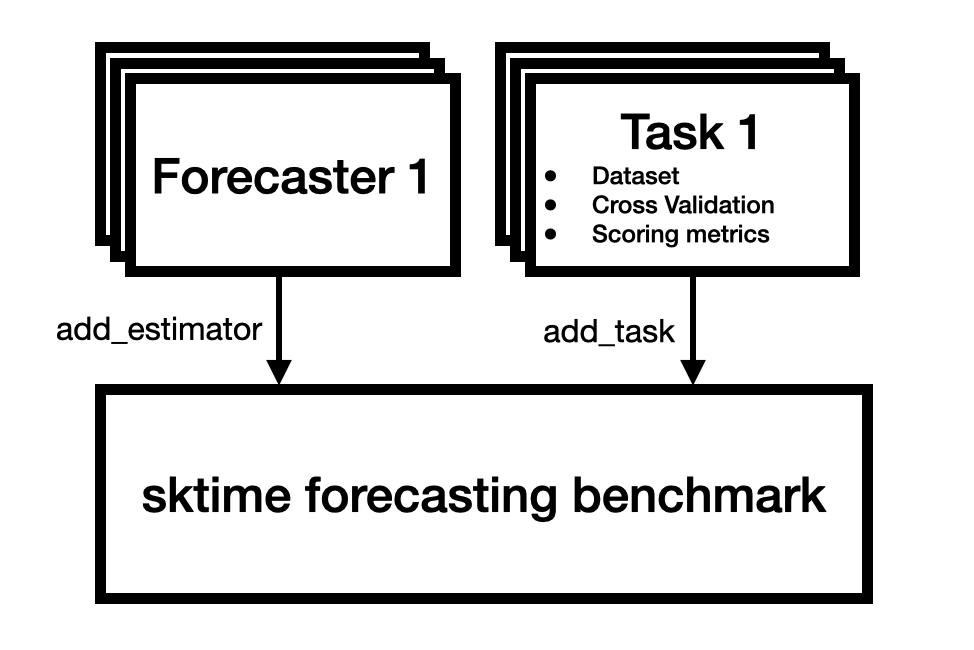
\includegraphics[width=.5\textwidth]{Figures/evaluationFramework.png}
    \caption{Benchmarking and evaluation framework}
    \label{fig:enter-label}
\end{figure}

\subsection{Prior Work}
The design principles of \texttt{sktime} draw inspiration from several established machine learning frameworks. Notably, \texttt{scikit-learn} in Python \cite{pedregosa2011scikit}, \texttt{mlr} in R \cite{bischl2016mlr}, and Weka \cite{hall2009weka} have pioneered the use of first-order specification languages and object-oriented design patterns for machine learning algorithms. 

\texttt{sktime} extends these foundational ideas by introducing specialized interfaces for time series forecasting, including both point and probabilistic forecasts. It also incorporates unique features such as:
\begin{itemize}
    \item Probabilistic forecasters and associated metrics interfaces
    \item Reproducibility patterns and APIs
    \item Meta-algorithms for enhanced composability
    \item Inhomogeneous API composition for flexible algorithmic design
\end{itemize}

Additionally, the \texttt{R/fable} package \cite{hyndman2020package} has contributed similar concepts specifically tailored to forecasting, which \texttt{sktime} has expanded upon or adapted to fit within its framework.

By leveraging and building upon these prior works, \texttt{sktime} offers a comprehensive and adaptable toolkit for time series forecasting, fostering reproducible research and facilitating extensive benchmarking and evaluation.
For a detailed analysis of design patterns in AI framework packages and innovations in \texttt{sktime}, see \cite{kiraly2021designing}.

\section{Algorithmic Setup} \label{methods}

In this section, we describe the forecasting algorithms used in our experiments. Our methods combine traditional forecasting models with uncertainty estimation wrappers, showcasing the benchmarking and model specification capabilities of \texttt{sktime}. This study serves as an invitation to the scientific Python community to engage and contribute to a more systematic study with reproducible specifications.

From a software perspective it is worth noting that \textbf{sktime} \cite{loning2019sktime, franz_kiraly_2024_11095261_sktime} contains multiple native implementations, including naive methods, all probability wrappers, and pipeline composition, but also provides a unified interface across multiple packages in the time series ecosystem:

\begin{itemize}
    \item \textbf{tsbootstrap} \cite{gilda_2024_10866090_tsbootstrap, gilda2024tsbootstrap}: A library for time series bootstrapping methods, integrated with \texttt{sktime}.
    \item \textbf{statsforecast} \cite{garza2022statsforecast}: A library for statistical and econometric forecasting methods, featuring the Auto-Theta algorithm.
    \item \textbf{statsmodels} \cite{seabold2010statsmodels}: A foundational library for statistical methods, used for the deseasonalizer and various statistical primitives.
\end{itemize}

This hybrid use of \texttt{sktime} as a framework covering first-party (itself), second-party (\texttt{tsbootstrap}), and third-party (\texttt{statsmodels}, \texttt{statsforecast}) locations is significant.
 Credit goes to the maintainers and implementers of these packages for implementing the contained algorithms that we can interface.

\subsection{Forecasting Pipeline}
Each forecaster is wrapped in a \texttt{Differencer} and a \texttt{Deseasonalizer} as preprocessing steps to improve stationarity. These preprocessors are necessary because some forecasters require the time series to be stationary (i.e., the properties of the time series at time $t+1$, $t+2$, ..., $t+n$ do not depend on the observation at time $t$ \cite{hyndman2018}) and non-seasonal.

\begin{itemize}
    \item \texttt{Differencer}: Computes first differences, which are inverted after forecasting by cumulative summing.
    \item \texttt{Deseasonalizer(sp=data\_sp)}: Removes the seasonal component, which is added back after forecasting. It estimates the trend by applying a convolution filter to the data, removing the trend, and then averaging the de-trended series for each period to return the seasonal component.
\end{itemize}

All used forecasters are point forecasters, i.e., for each time step they provide one value (point), and no information about the uncertainty of the forecast. Thus, they are combined with one of the probabilistic wrappers to generate prediction intervals or quantile forecasts.

\begin{figure}
    \centering
    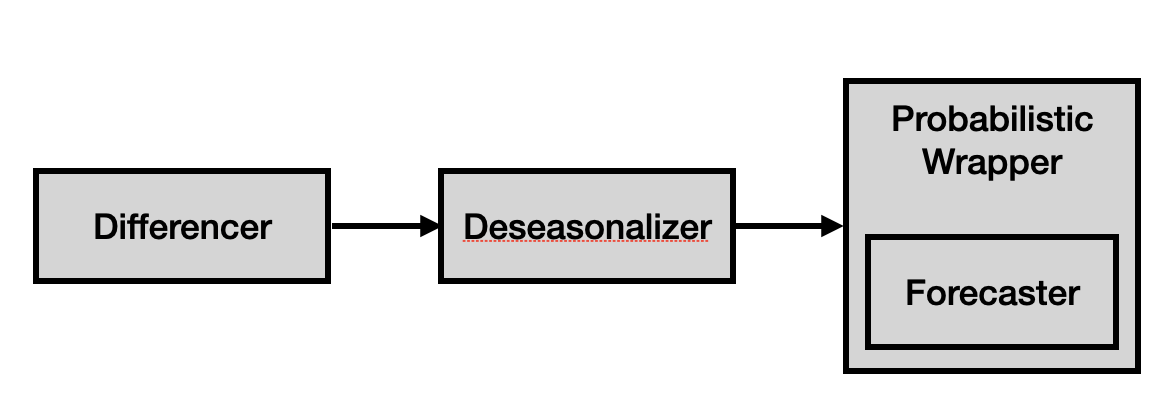
\includegraphics[width=\textwidth]{Figures/Pipeline.png}
    \caption{The forecasting pipeline used for all the forecasters}
    \label{fig:pipeline}
\end{figure}

The partial pipeline specification, illustrated in Figure \ref{fig:pipeline}, is:

\begin{verbatim}
Differencer() * Deseasonalizer(sp=data_sp) * wrapper(forecaster)
\end{verbatim}

where variable parts are \texttt{wrapper}, \texttt{forecaster}, and \texttt{data\_sp}. These components are varied as described below.
Note the code for running the whole benchmark is provided in the Section~\ref{experiment}.

\subsection{Component Forecasting Models}

We use several component forecasting models in this study, each with unique characteristics:

\begin{itemize}
    \item \texttt{NaiveForecaster(strategy, sp)}: Uses simple heuristics for forecasting. The \texttt{strategy} parameter allows selecting the type of algorithm:
    \begin{itemize}
        \item \texttt{mean}: Uses the mean of the last \(N\) values, with seasonal periodicity \texttt{sp} if passed.
        \item \texttt{last}: Uses the last observed, with seasonal periodicity \texttt{sp} if passed.
        \item \texttt{drift}: Fits a line between the first and last values of the considered window and extrapolates forward.
    \end{itemize}

    \item \texttt{StatsForecastAutoTheta(sp)}: A variant of the Theta model of \cite{Assimakopoulos2000} with automated parameter tuning, from the \texttt{statsforecast} library.
    
\end{itemize}

\subsection{Probabilistic Wrappers}
We use the following probabilistic wrappers to enhance the forecasting models:

\begin{itemize}
    \item \texttt{ConformalIntervals(forecaster, strategy)}: Uses conformal prediction methods \cite{Stankeviciute2021} to produce non-parametric prediction intervals. Variants of the method are selected by the \texttt{strategy} parameter: \textbf{Empirical} and \textbf{Empirical Residual} use training quantiles, with the latter using symmetrized residuals. \textbf{Conformal} implements the method of \cite{Stankeviciute2021}, and \textbf{Conformal Bonferroni} applies the Bonferroni correction.
    \item \texttt{BaggingForecaster(bootstrap\_transformer, forecaster)}: Provides probabilistic forecasts by bootstrapping time series and aggregating the bootstrap forecasts \cite{hyndman2018, bergmeir2016}. The \texttt{BaggingForecaster} takes a bootstrap algorithm \texttt{bootstrap\_transformer}, a first-class object in \texttt{sktime}. Various bootstrap algorithms with their parameters are applied in the study.
    \item \texttt{NaiveVariance(forecaster)}: Uses a sliding window to compute backtesting residuals, aggregated by forecasting horizon to a variance estimate. The mean is obtained from the wrapped forecaster, and variance from the pooled backtesting estimate.
    \item \texttt{SquaringResiduals(forecaster, residual\_forecaster)}: Uses backtesting residuals on the training set, squares them, and fits the \texttt{residual\_forecaster} to the squared residuals. Forecasts of \texttt{residual\_forecaster} are used as variance predictions, with mean predictions from \texttt{forecaster}, to obtain a normal distributed forecast. In this study, \texttt{residual\_forecaster} is always \texttt{NaiveForecaster(strategy="last")}.
\end{itemize}

\subsection{Bootstrapping Techniques}
Bootstrapping methods generate multiple resampled datasets from the original time series data, which can be used as part of wrappers to estimate prediction intervals or predictive distributions. In this study, we use bootstrap algorithms from \texttt{tsbootstrap} \cite{gilda2024tsbootstrap, gilda_2024_10866090_tsbootstrap}, \texttt{sktime} \cite{franz_kiraly_2024_11095261_sktime}, and \texttt{scikit-learn} \cite{pedregosa2011scikit} compatible framework library dedicated to time series bootstrap algorithms. \texttt{sktime} adapts these algorithms via the \texttt{TSBootstrapAdapter}, used as \texttt{bootstrap\_transformer} in \texttt{BaggingForecaster}.

\begin{itemize}
    \item \texttt{MovingBlockBootstrap}: Divides the time series data into overlapping blocks of a fixed size and resamples these blocks to create new datasets. The block size is chosen to capture the dependence structure in the data.
    \item \texttt{BlockDistributionBootstrap}: Generates bootstrapped samples by fitting a distribution to the residuals of a model and then generating new residuals from the fitted distribution. This method assumes that the residuals follow a specific distribution, such as Gaussian or Poisson, and handles dependencies by resampling blocks of residuals.
    \item \texttt{BlockResidualBootstrap}: Designed for time series data where a model is fit to the data, and the residuals (the difference between the observed and predicted data) are bootstrapped. This method is particularly useful when a good model fit is available for the data. The bootstrapped samples are created by adding the bootstrapped residuals to the model's fitted values.
    \item \texttt{BlockStatisticPreservingBootstrap}: Generates bootstrapped time series data while preserving a specific statistic of the original data. This method handles dependencies by resampling blocks of data while ensuring that the preserved statistic remains consistent.
\end{itemize}

In this study, these bootstrapping techniques are used to estimate the distribution of forecasts and generate robust prediction intervals and predictive distributions as part of the \texttt{BaggingForecaster}.

\subsection{Evaluation Metrics}
We evaluate the performance of our forecasting models using the following metrics:

\begin{itemize}
    
    \item \texttt{CRPS} - Continuous Ranked Probability Score \cite{matheson1976} measures the accuracy of probabilistic forecasts by comparing the predicted distribution to the observed values. The CRPS for a real-valued forecast distribution $d$ and an observation $y$ can be defined as:
    \[
    \text{CRPS}(d, y) = \mathbf{E} \left[ \left| X - y \right| \right] - \frac{1}{2} \mathbf{E} \left[ \left| X - X' \right| \right],
    \]
    where $X$ and $X'$ are independent random variables with distribution $d$.
    
    \item \texttt{PinballLoss} - the pinball loss, also known as quantile loss \cite{pinball_loss}, evaluates the accuracy of quantile forecasts by penalizing deviations from the true values based on specified quantiles.
    For quantile forecasts $\hat{q}_1, \dots, \hat{q}_k$ at levels $\tau_1, \dots, \tau_k$ and an observation $y$, the Pinball Loss is defined as:

    \begin{equation}
    L(\hat{q}, y) = \frac{1}{k} \sum_{i=1}^k \max \left(\tau_i (y - \hat{q}_i), (1 - \tau_i) (\hat{q}_i - y)\right)
    \end{equation}

    The experiment uses the Pinball Loss at quantiles 0.05, and 0.95.

    \item \texttt{AUCalibration} - The Area between the calibration curve and the diagonal assesses how well the prediction intervals capture the true values. For observations $y_1, \dots, y_n$ and corresponding distributional predictions with quantile functions $Q_1, \dots, Q_n$ (where $Q_i = F^{-1}_i$ for the cdf $F_i$), the AUCalibration is defined as:
    \begin{equation}
    \mbox{AUC} (Q_:, y_:) = \frac{1}{N} \sum_{i=1}^N \left| c_{(i)} - \frac{i}{N}\right|,
    \end{equation}
    where $c_i := Q_i(y_i),$ and $c_{(i)}$ is the $i$-th order statistic of $c_1, \dots, c_N$.

    \item \texttt{IntervalWidth} - width of prediction intervals, or sharpness measures the concentration of the prediction intervals. More concentrated intervals indicate higher confidence in the forecasts. Sharpness is desirable because it indicates precise predictions. Sharpness is calculated as the average width of the prediction intervals.
    \item \texttt{EmpiricalCoverage} - Empirical coverage measures how much of the observations are within the predicted interval. It is computed as the proportion of observations that fall within the prediction, providing a direct measure of the reliability of the intervals. A prediction interval ranging from the 5th to the 95th quantile should cover 90\% of the observations. I.e., the empirical coverage should be close to 0.9.
    \item \texttt{runtime} - Besides metrics that assess the quality of the forecast, average runtime for an individual fit/interence run is also reported. Runtime measures the computational efficiency of the forecasting methods, which is crucial for practical applications.
 
\end{itemize}

\begin{table}[h]
    \centering
    \footnotesize
    \caption{To perform the evaluation, we used three datasets. Due to the different frequencies and lengths, we used different parameters for the Sliding Window Splitter to create the cross-validation folds. This table presents the parameters used for each dataset.}
    \label{tab:evaluation_splits}
    \begin{tabularx}{\textwidth}{X|X|X|X|X|X|X}
         \toprule
        Dataset & Forecast Horizon & Step Width & Window Size & Cutout Period & Number of Folds & Seasonal Length \\ \midrule
        Australian Electricity Demand & 48 & 1440 & 1440 & Last Year & 12 & 48 \\ 
        Sunspot Activity & 28 & 395 & 365 & Last 40 Years & 12 & 1\\
        US Births & 28 & 395 & 365 & Whole Time Series & 12 & 1 \\
        \bottomrule
    \end{tabularx}
\end{table}


\begin{table}[h]
    \centering
    \footnotesize
    \caption{The code instantiation of the cross-validation splits used for the evaluation on the three datasets. The parameters are taken from Table \ref{tab:evaluation_splits}.}
    \label{tab:cv_splits}
    \begin{tabularx}{\textwidth}{X|X}
         \toprule
        Dataset & CV splitter \\ \midrule
        Australian Electricity Demand & \texttt{SlidingWindowSplitter(step_length=48*30, window_length=48*30,fh=range(48))} \\  
        Sunspot Activity & \texttt{SlidingWindowSplitter(step_length=395, window_length=365,fh=range(28))}\\
        US Births & \texttt{SlidingWindowSplitter(step_length=395, window_length=365,fh=range(28))}\\
        \bottomrule
    \end{tabularx}
\end{table}



\section{Experiments} \label{experiments}
In this section, we describe the experimental setup, the datasets, the evaluation metrics, and the experimental procedures. We explain how the experiments are designed to compare the performance of different forecasting methods.

% \subsection{Software Setup}
% The software used in our experiments includes:

% \begin{itemize}
%     \item \textbf{sktime:} A library for machine learning with time series data.
%     \item \textbf{tsbootstrap:} A library for time series bootstrapping methods.
%     \item \textbf{Statsforecast:} A library for statistical and econometric forecasting methods.
%     \item \textbf{kotsu:} A library for benchmarking and validating machine learning models.
% \end{itemize}

\subsection{Experimental Setup}
To perform the benchmarking study, we use the framework described in Section~\ref{methods}. The benchmarking compares different probabilistic wrappers on different datasets and with different forecasters regarding CRPS, Pinball Loss, AUCalibration, and Runtime. 

To enable easy replication of the experiments, we provide for each used forecaster, and wrapper the hyperparameters by providing the used Python object instantiation in Table~\ref{tab:hyperparams}. These hyperparameter depend on the dataset, especially, the seasonal periodicity (sp) is chosen based on the dataset. This parameter as well as the other dataset related parameter required to create the cross validation folds used for the evaluation are described in Table~\ref{tab:evaluation_splits}. To create the cross validation folds, we use the \texttt{SlidingWindowSplitter} from \texttt{sktime}. The instantiation of the splitter for each dataset is shown in Table~\ref{tab:cv_splits}. Figure~\ref{fig:splits} is showing the resulting cross validation folds for the tree datasets.

\begin{figure}
    \centering
    \begin{subfigure}{1\textwidth}
        \centering
        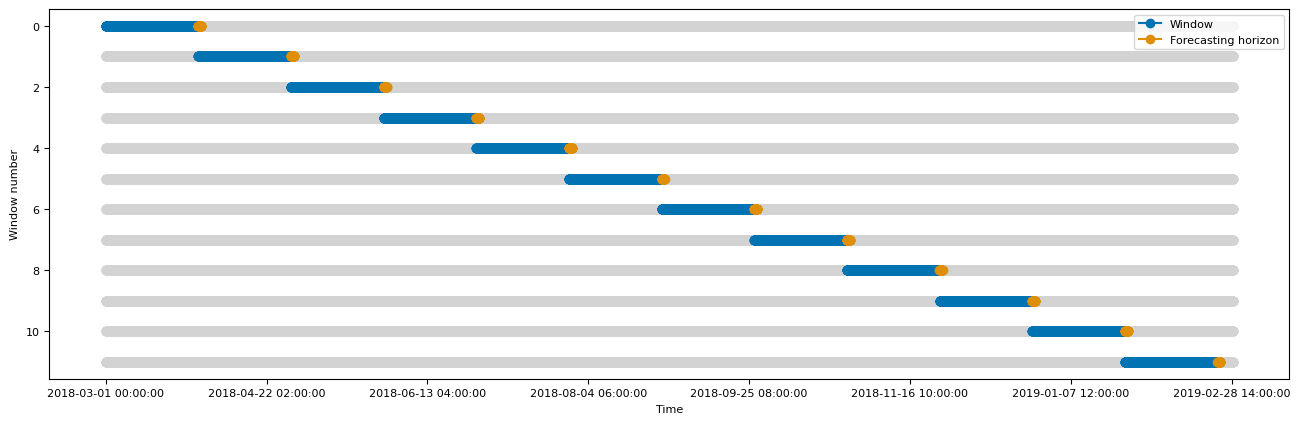
\includegraphics[width=\textwidth]{Figures/AusElecSplit.png}
        \caption{Australian Electricity Demand}
        \label{fig:aus_split}
    \end{subfigure}

    \begin{subfigure}{1\textwidth}
        \centering
        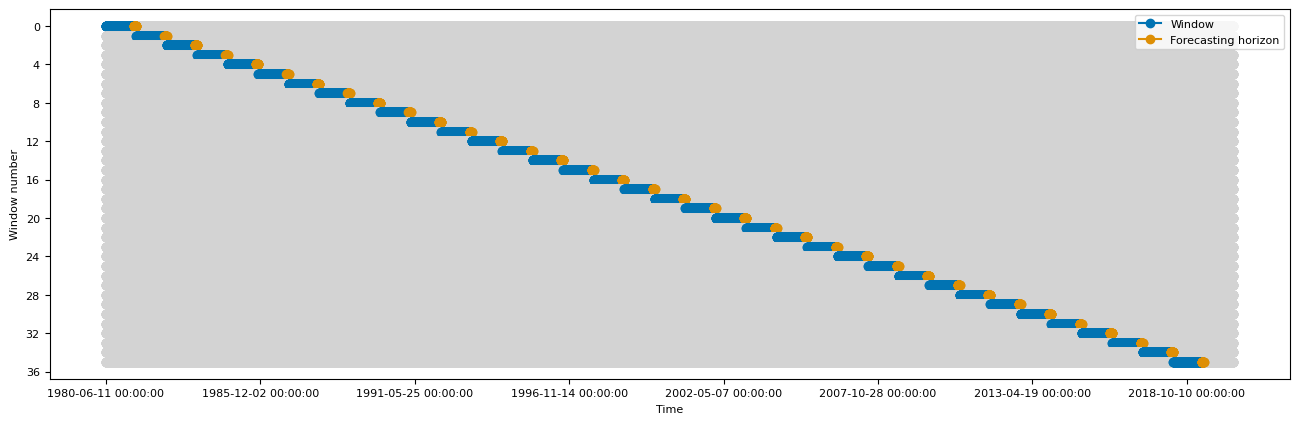
\includegraphics[width=\textwidth]{Figures/SunspotSplit.png}
        \caption{Sunspot Activity}
        \label{fig:sunspot_split}
    \end{subfigure}

    \begin{subfigure}{1\textwidth}
        \centering
        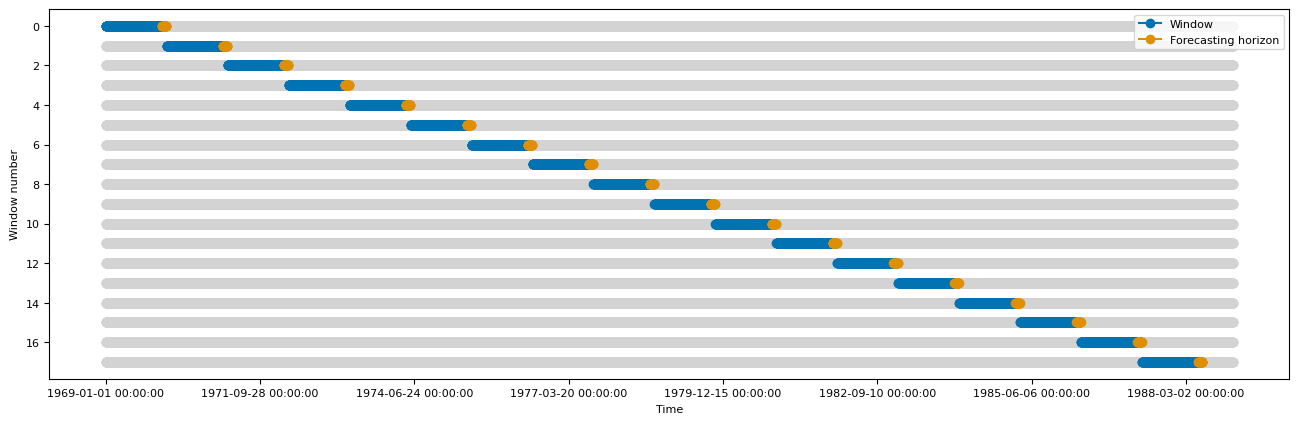
\includegraphics[width=\textwidth]{Figures/USBirthSplit.png}
        \caption{US Births}
        \label{fig:usbirth_split}

    \end{subfigure}
    \caption{The splits used for the evaluation on the three datasets. Blue indicates the training data, and orange indicates the test data. The splits are created using the parameters from Table~\ref{tab:evaluation_splits} and Table~\ref{tab:cv_splits}}
    \label{fig:splits}
\end{figure}

\subsection{Datasets} \label{datasets}
We evaluate our forecasting methods and probabilistic wrappers on several diverse time series datasets, each offering unique characteristics:

\begin{itemize}
    \item \textbf{Australian Electricity Demand \cite{Godahewa2021Australian}}: Half-hourly electricity demand data for five series in Australia, useful for high-frequency data evaluation.
    \item \textbf{Sunspot Activity \cite{Godahewa2021Sunspot}}: Weekly observations of sunspot numbers, ideal for testing forecasting robustness on long-term periodic patterns.
    \item \textbf{US Births \cite{Godahewa2021USBirth}}: Daily birth records in the United States, with a clear seasonal pattern, suitable for daily data performance assessment.
\end{itemize}


% \begin{itemize}
%     \item \textbf{Data Preprocessing:} We preprocess the datasets by handling missing values, normalizing the data, and splitting it into training and test sets.
%     \item \textbf{Model Training:} We train each forecasting model on the training set. For ARIMA models, we use the AutoARIMA function to automatically select the best hyperparameters. For naive forecasters, we use the mean, last, and drift methods as described earlier.
%     \item \textbf{Bootstrapping:} We apply the Moving Block Bootstrap (MBB) technique, as well as other blocked bootstrapping techniques, to generate multiple resampled datasets from the training data.
%     \item \textbf{Prediction Interval Generation:} We use the bootstrapped datasets to generate prediction intervals for each forecasting model.
%     \item \textbf{Evaluation:} We evaluate the performance of the forecasting models and probabilistic wrappers using the metrics described in the Methodology section.
% \end{itemize}

\begin{table}[]
    \centering    \caption{
    The table lists the specification strings for the estimators used in the study. Note that a full pipeline consists of pre-processing, wrapper, and base forecaster, as detailed in section \ref{methods}. \\
    Some of the parameters are determined by the used dataset: sp is 48 for the Autralian Electricity Dataset and 1 for the other. The sample\_freq is 0.005 for the Australian Electricity Dataset and 0.1 for the other.\\}
    \label{tab:hyperparams}
    \footnotesize
    \begin{tabular}{p{2.5cm}p{4cm}|p{7.5cm}}
    \toprule  
         Role & Name &  Hyperparameters \\ \midrule
         Base Forecaster & Naive last &  \texttt{NaiveForecaster(strategy="last", sp=sp)}\\
         Base Forecaster &  Naive mean &  \texttt{NaiveForecaster(strategy="mean", sp=sp)}\\
         Base Forecaster & Naive drift &  \texttt{NaiveForecaster(strategy="drift", sp=sp)}\\ 
         Base Forecaster & Theta &   \texttt{StatsForecastAutoTheta(season\_length=sp)} \\ \midrule
         Wrapper & CI Empirical & \texttt{ConformalIntervals(forecaster, sample\_frac=sample\_frac)} \\
         Wrapper & CI Empirical residuals & \texttt{ConformalIntervals(forecaster, sample\_frac=sample\_frac, method="empirical\_residual")} \\
         Wrapper & CI Conformal & \texttt{ConformalIntervals(forecaster, sample\_frac=sample\_frac, method="conformal")} \\
         Wrapper & CI Bonferroni & \texttt{ConformalIntervals(forecaster, sample\_frac=sample\_frac, method="conformal\_bonferroni")} \\
         Wrapper & BaggingForecaster & \texttt{BaggingForecaster(ts\_bootstrap\_adapter, forecaster))} \\
         Wrapper & Naive Variance & \texttt{NaiveVariance(forecaster, initial\_window=14*sp))}\\
         Wrapper & Squaring Residuals & \texttt{SquaringResiduals(forecaster, initial\_window=14*sp))}  \\ \midrule
         Forecasting Pipeline & Pipeline & \texttt{Differencer(1) * Deaseasonalizer(sp=sp) * Wrapper} \\ \midrule
        
         ts\_bootstrap\_adapter & TSBootstrapAdapter & \texttt{TSBootstrapAdapter(tsbootsrap)} \\
         %Differencer& Differencer &  \\
         %Deseasonalizer & Deseasonalizer &  \\ 
         \midrule
 
         tsbootstrap & Moving Block Bootstrap & \texttt{MovingBlockBootstrap()} \\
         tsbootstrap & Block Residual Bootstrap & \texttt{BlockDistributionBootstrap()} \\
         tsbootstrap & Block Statistic Preserving Bootstrap & \texttt{BlockStatisticPreservingBootstrap()} \\
         tsbootstrap & Block Distribution Bootstrap & \texttt{BlockDistributionBootstrap()}\\

         \bottomrule
         
    \end{tabular}
\end{table}

% \subsection{Evaluation Metrics}
% The evaluation metrics used in this study include Continuous Ranked Probability Score (CRPS), Pinball Loss, Calibration, Sharpness, Empirical Coverage, and Runtime. These metrics provide a comprehensive assessment of the accuracy, reliability, and computational efficiency of the probabilistic forecasts.

% \subsection{Experimental Procedure}
% We conduct experiments on each dataset by following the experimental setup described above. For each dataset, we train the forecasting models on the training set and generate prediction intervals using the bootstrapped datasets. We then evaluate the performance of the models and probabilistic wrappers on the test set using the evaluation metrics.


\subsection{Results} \label{results}
In this section, we present the results of our experiments. We evaluate the performance of the forecasting methods combined with probabilistic wrappers on the datasets described in Section \ref{datasets}. 
%Our primary focus is on the accuracy and reliability of the prediction intervals generated by these methods.
To increase the conciseness, we calculated the rank of each probabilistic wrapper for each combination of forecaster, metric, and dataset. Afterwards, for each metric, probabilistic wrapper and dataset, we have calculated the average across all forecasters and time series. In the following, we present the results for each dataset separately. 


\subsubsection{Performance on Australian Electricity Demand}
The results for the Australian electricity demand dataset are summarized in Table \ref{table:aus_elec_results}. We compare the performance of different forecasting models and probabilistic wrappers using the previously described evaluation metrics. 

The ranked based evaluation show that diverse results regarding the different metrics. E.g. while CI Empirical Residual performs best on CRPS, it is only mediocre regarding the Pinball Loss and the AUCalibration. On PinballLoss, the best method is CI Empirical and on AUCalibration, it is Squaring Residuals. Regarding the runtime, the fastest method is the fallback probabilistic prediction of the base forecaster. The slowest methods are NaiveVariance and SquaringResiduals. Furthermore, it seems that the ConformalIntervals are slightly faster than the BasggingForecasters.

\begin{table}[h]
    \centering
    \caption{Performance of forecasting methods on the Australian electricity demand dataset}
    \label{table:aus_elec_results}
\begin{tabular}{lrrrr}
\toprule
Wrapper & CRPS & Pinball Loss & AUCalibration & Runtime \\
\midrule
Fallback & 9.45 & 9.66 & 5.61 & 1.00 \\
Naive Variance & 7.75 & 7.20 & 7.15 & 10.00 \\
Squaring Residuals & 7.45 & 6.20 & 5.05 & 11.00 \\
Block Distribution Bootstrap & 4.08 & 3.15 & 6.82 & 7.83 \\
Block Residual Bootstrap & 4.30 & 5.58 & 5.84 & 8.32 \\
Block Statistic Preserving Bootstrap & 4.25 & 5.87 & 6.15 & 7.29 \\
Moving Block Bootstrap & 6.12 & 6.51 & 4.26 & 6.00 \\
CI Conformal & 5.75 & 5.40 & 5.69 & 3.92 \\
CI Empirical & 3.79 & 2.63 & 6.97 & 3.30 \\
CI Empirical Residual & 2.37 & 5.42 & 5.35 & 3.49 \\
CI Bonferroni  & 10.50 & 8.05 & 6.70 & 3.70 \\
\bottomrule
\end{tabular}

\end{table}

\subsubsection{Performance on Sunspot Activity}
Table \ref{table:sunspot_results} shows the performance of our methods on the sunspot activity dataset. The long-term periodic patterns in this dataset provide a challenging test for our forecasting models.

The ranked based evaluation show that BaggingForecaster with the Block Distribution Bootstrap scores clearly best regarding the CRPS and Pinball Loss, and AUCalibration. Regarding the runtime, the fastest method is the fallback probabilistic prediction of the base forecaster. The slowest methods are NaiveVariance and SquaringResiduals. 
Furthermore, it seems that the ConformalIntervals are slightly faster than the BasggingForecasters. 
\begin{table}[h]
    \centering
    \caption{Performance of forecasting methods on the sunspot activity dataset}
    \label{table:sunspot_results}
\begin{tabular}{lrrrr}
\toprule
Wrapper & CRPS & PinballLoss & AUCalibration & Runtime \\
\midrule
Fallback & 9.00 & 7.25 & 9.50 & 1.00 \\
Naive Variance & 6.50 & 6.25 & 7.75 & 10.00 \\
Squaring Residuals & 8.00 & 8.00 & 4.75 & 11.00 \\
Block Distribution Bootstrap & 1.00 & 1.00 & 3.00 & 7.25 \\
Block Residual Bootstrap & 6.00 & 6.25 & 5.00 & 6.75 \\
Block Statistic Preserving Bootstrap & 5.50 & 7.00 & 2.50 & 6.25 \\
Moving Block Bootstrap & 5.75 & 5.75 & 7.50 & 5.00 \\
CI Conformal & 4.75 & 4.50 & 6.75 & 4.50 \\
CI Empirical & 5.50 & 4.00 & 7.25 & 4.50 \\
CI Empirical Residual & 3.50 & 8.00 & 6.25 & 4.25 \\
CI Bonferroni  & 10.50 & 8.00 & 5.75 & 5.50 \\
\bottomrule
\end{tabular}


\end{table}

\subsubsection{Performance on US Births}
The results for the US births dataset are presented in Table \ref{table:us_births_results}. This dataset, with its clear seasonal pattern, allows us to assess the models' ability to handle daily data.
The ranked based evaluation show that BaggingForecaster with the Block Distribution Bootstrap scores best regarding the CRPS and Pinball Loss. 
Regarding the AUCalibration, the best score is achieved by CI Conformal. Regarding the runtime, the fastest method is the fallback probabilistic prediction of the base forecaster. The slowest methods are NaiveVariance and SquaringResiduals. Furthermore, it seems that the ConformalIntervals are slightly faster than the BasggingForecasters. 

\begin{table}[h]
    \centering
    \caption{Performance of forecasting methods on the US births dataset}
    \label{table:us_births_results}
\begin{tabular}{lrrrr}
\toprule
Wrapper & CRPS & PinballLoss & AUCalibration & Runtime \\
\midrule
Fallback & 9.25 & 9.50 & 7.88 & 1.00 \\
Naive Variance & 6.25 & 5.75 & 6.25 & 10.00 \\
Squaring Residuals & 9.50 & 8.50 & 6.50 & 11.00 \\
Block Distribution Bootstrap & 1.00 & 1.00 & 8.25 & 7.25 \\
Block Residual Bootstrap & 3.75 & 5.75 & 5.50 & 7.00 \\
Block Statistic Preserving Bootstrap & 5.50 & 6.00 & 7.38 & 6.25 \\
Moving Block Bootstrap & 5.75 & 5.25 & 5.12 & 4.75 \\
CI Conformal & 6.00 & 6.00 & 4.75 & 4.25 \\
CI Empirical & 5.50 & 4.50 & 4.88 & 4.75 \\
CI Empirical Residual & 3.00 & 6.00 & 5.00 & 5.25 \\
CI Bonferroni  & 10.50 & 7.75 & 4.50 & 4.50 \\
\bottomrule
\end{tabular}

\end{table}


\section{Discussion and Conclusion} \label{conclusion}
Our experiments demonstrate that the benchmarking framework in \texttt{sktime} provides an easy-to-use solution for reproducible benchmarks. We showed this by conducting simple benchmark studies of probabilistic wrappers for point forecasts on three different systems.

Regarding our benchmark study, we note that this is a limited study primarily aimed at showcasing the capabilities of the proposed framework. Therefore, future work should include a comprehensive hyperparameter search to identify the best parameters for the probabilistic wrappers. Additionally, further bootstrapping methods need to be explored, as well as other wrappers such as generative neural networks, including Generative Adversarial Networks, Variational Autoencoders, or Invertible Neural Networks \cite{phipps2024, wang2020}.

Besides extending the range of wrappers, we also plan to include additional point forecasters as base models, such as AutoARIMA, in our study. Furthermore, the number of examined datasets should be expanded to provide a more comprehensive evaluation. Finally, we did not perform a grid search on the hyperparameters for the wrappers, which means that with different hyperparameters, their performance and runtime might change.

In conclusion, the \texttt{sktime} evaluation modules enable the performance of reproducible forecasting benchmarks. We demonstrated its applicability in a small benchmarking study that compares different probabilistic wrappers for point forecasters. In future work, we aim to collaborate with the scientific community to integrate more wrappers and conduct a broader benchmark study on this topic.

\bibliographystyle{alpha}
\bibliography{sample}
